\documentclass[12pt]{article} 	% Type de document & taille de police
\usepackage[margin=2.53cm]{geometry}  % Marges normales de Word
\usepackage[french]{babel}  % Langue
\usepackage[utf8]{inputenc}  % Saisi du texte : permet les accents
\usepackage[T1]{fontenc} 	% Encodage du document
\setlength{\parindent}{0pt}  % Pas d'indentation
\setlength{\parskip}{1em}  % Passer une ligne après chaque paragraphe
\usepackage{hyperref}	% Inclure les liens
\usepackage{graphicx}	% Inclure des images
\topskip0pt  % Permet \vspace*{\fill} pour centrer verticalement
\usepackage{xcolor} % Texte coloré
\usepackage{enumitem}
\usepackage[printonlyused]{acronym}
\usepackage{multicol} %<<<<<<<<<<<
\usepackage{amsmath, amstext, amsfonts,amssymb}
\usepackage{tikz}
\usepackage{commath}
\usepackage{booktabs}
\usepackage{multirow}
\newlist{abbrv}{itemize}{1}
\setlist[abbrv,1]{label=,labelwidth=1in,align=parleft,itemsep=0.1\baselineskip,leftmargin=!}
\newcommand{\notation}[1]{\textcolor{blue}{{#1}}}

\newif\ifnotes
\makeatletter
\newcommand{\note}[1]{\@bsphack\ifnotes{#1}\fi\@esphack}
\makeatother
\newcommand{\nonotes}{\notesfalse}
\newcommand\capitalLetter[1]{\textsc{\MakeLowercase{#1}}}


%%%%%%%%%%%%%%%%%%%%% Section à remplir %%%%%%%%%%%%%%%%%%%%%
\newcommand\titreDuCours{Stage en génie logiciel III}
\newcommand\sigleCoursStage{GLO-2531}
\newcommand\session{Été 2042}
\newcommand\acronymeDuBac{GLO}

\newcommand\titreStagiaire{Nom du stagiaire}
\newcommand\titreStage{Titre du stage}
\newcommand\nomCompagnie{Nom de la compagnie}

\newcommand\dateRemise{42 avril 2042}
\newcommand\prenomStagiaire{Lesta}
\newcommand\nomStagiaire{Giaire}
\newcommand\idul{123 456 789}

\newcommand\prenomSuperviseur{Lesuper}
\newcommand\nomSuperviseur{Viseur}
\newcommand\titreSuperviseur{Titre De Mon superviseur}

% Changer si la page de présentation ne tient pas sur une page
\newcommand\distanceEnteteEtNomStage{4cm}
\newcommand\distanceTypeRapportEtDestinataire{5cm}

% mettre \notesfalse si vous voulez supprimer les notes sinon \notestrue
\notestrue
%\notesfalse
%%%%%%%%%%%%%%%%%%%%%%%%%%%%%%%%%%%%%%%%%%%%%%%%%%%%%%%%%%%%%

\begin{document}

\thispagestyle{empty}
\begin{minipage}[t]{8.5cm}
    \vspace{0pt}
    \begin{flushleft}
        \hspace{-1cm}
\includegraphics[width=5cm]{img/UL-FSG-C-g-3lignes.png}\\
    \end{flushleft}
\end{minipage}
\begin{minipage}[t]{8.5cm}
    \begin{flushright}
        \hspace*{2cm} \\
        \hspace*{1cm}\titreDuCours\\
        \hspace*{1cm}\sigleCoursStage\\
        \hspace*{1cm}\session\\
        \hspace*{1cm}Baccalauréat en {\acronymeDuBac}\\
    \end{flushright}
\end{minipage}

\vspace{\distanceEnteteEtNomStage}
\begin{center}
    
    \fontsize{14.4}{14.4}\large \textbf{Rapport de stage}\\
    \vspace{1cm}
    \large {\titreStage}  \\
\vspace{0.2cm}
    {\nomCompagnie} \\
    \vspace{\distanceTypeRapportEtDestinataire}
    \fontsize{14.4}{14.4}\textbf {Destinataire}\\
    \large Département des stages  - Direction de la Faculté des sciences et de génie \\
\end{center}
\vspace{2cm}
\begin{flushleft}
    Date de remise : {\dateRemise}
\end{flushleft}

\par\noindent\rule{\textwidth}{0.4pt}
\begin{minipage}[t]{6cm}
    \begin{flushleft}
        \textbf {\prenomStagiaire~\nomStagiaire}\\
        \idul
    \end{flushleft}
\end{minipage}
\begin{minipage}[t]{10cm}
    \begin{flushright}
        \hspace*{1cm}\textbf {\prenomSuperviseur~\nomSuperviseur~- \titreSuperviseur} \\
    \end{flushright}
\end{minipage}

\newpage
\pagenumbering{Roman}

\addcontentsline{toc}{section}{\numberline{}Résumé}
\textbf{Résumé} {\note{{\notation{(5\% de la note finale)}}

Le résumé est le condensé de l’ensemble du rapport. Il doit permettre au lecteur de comprendre l’essentiel de votre stage sans avoir lu la totalité du rapport. Un résumé doit présenter : le but et la nature du travail, les méthodologies utilisées, les principaux résultats et les principales conclusions. Il énumère en outre l'entreprise d'accueil, la période de stage et les tâches du stagiaire.

Exemple : « Ce rapport présente le travail effectué par {\prenomStagiaire}
    {\nomStagiaire} dans le cadre du stage de formation en entreprise, dans le département (de ...) de la compagnie {\nomCompagnie}, pendant la période (du ...). Le stage a consisté à ... » }}                % résumé français

\newpage
% Remerciements
\addcontentsline{toc}{section}{\numberline{}Remerciements}
\textbf{Remerciements}
\begin{flushleft}
    Je tiens à remercier {\prenomSuperviseur} {\nomSuperviseur}...
\end{flushleft}
\vspace*{\fill} 


\newpage
% Table des matières
\tableofcontents


\newpage
% Listes des tableaux
\listoftables


\newpage
% Table des figures
\listoffigures


\newpage
\addcontentsline{toc}{section}{\numberline{}Liste de symboles et abréviations}
\textbf{Liste de symboles et abréviations}\\
\note{
\begin{multicols}{2}
\begin{acronym}[VBLAST]  % longest acronym to fix width
    \acro{LS}{least squares}\acused{LS}
    \acro{WARP}{Wireless Open-Access Research Platform (Plate-forme de recherche sans fil en libre accès)}\acused{WARP}
    \acro{VBLAST}{Vertical Bell Laboratories Layered Space-Time ()}\acused{VBLAST}
    
\end{acronym}
\end{multicols}
\acresetall

Lors de la première utilisation, vous devez utiliser \textbackslash ac\{WARP\} comme \ac{WARP} qui permet d'écrire l'abréviations au complet. Puis après la première utilisation, vous pouvez introduire votre abréviation ainsi  \textbackslash acs \{WARP\} pour obtenir \acs{WARP}. Si vous n'énumérez pas une abréviation, elle ne s'affichera pas dans la liste ci-dessus. Par exemple, si je utilise seulement \acs{WARP} et \ac{VBLAST}, LS ne s'affichera pas. Pensez à traduire vos abréviations si elles sont en anglais. Pour le cas de \acs{VBLAST}, il s'agit du nom d'un algorithme de détection, vous pouvez le laisser en anglais.}

\break


\newpage
\pagenumbering{arabic}

\section{Introduction}
\leavevmode
\note{\notation{(10\% de la note finale)} L'introduction doit être au maximum d'une page. La problématique doit être au présent, les hypothèses (s'il y en a), au conditionnel. Le mandat et le contenu sont au présent.}

\subsection{Présentation personnelle} 
\note{\notation{(3\% de la note finale)}Présentation personnelle: nom, programme, cheminement scolaire et professionnel dont l’avancement dans le programme et les stages.}

\subsection{Présentation de l'organisation}
\note{\notation{(3\% de la note finale)}Présentation de l’organisation : nom de l’entreprise ou du centre de recherche, secteur d’activité, mission, taille, services / produits, effectifs, localisation.}

\subsection{Présentation du stage et de son environnement}
\note{\notation{(3\% de la note finale)} Présentation du/des projet(s) dans le cadre de la mission de l'organisation ou du domaine de recherche, titre du stagiaire, environnement de travail, taille de l'équipe, Période du stage, type d'encadrement : superviseur (titre et  fonction), lieu de travail, etc. }


\newpage
\section{Responsabilités et tâches du stagiaire}
\leavevmode
\note{\notation{(20\% de la note finale)} Le temps de cette section est le présent. Le contenu principal du rapport qui décrit toutes les étapes franchies et les moyens mis de l'avant pour solutionner les différentes problématiques, une validation des résultats obtenus et la formulation de recommandations pour le futur. Comment la formation en milieu pratique sera porteuse pour la suite des  études de baccalauréat ou pour la fin de la formation universitaire.

{\bfseries{Il est fortement recommandé d'inclure dans cette section des figures, des tableaux, des schémas, des photos ou autres éléments visuels sous peine de perdre des points (jusqu'à \notation{(10\% de la note finale)}).}} Cependant ces éléments doivent apparaître dans le corps du rapport en autant que cela occupe une place raisonnable. Chaque figure et tableau doit correctement être expliqué de manière à être compris indépendamment du texte. Si une section de texte comporte des calculs, croquis de diagrammes, des plans, spécifications techniques ou autres éléments de rapport nécessitant plus d'une demi-page, alors il est souvent préférable d’inclure ces divers éléments en annexe. En fait, pour le corps du texte, on se limite à citer en référence l’élément en question et à décrire les principales hypothèses ou explications nécessaires à la compréhension de ce qui est présenté, les résultats obtenus et la conclusion à laquelle on arrive, interprétation du concept ou autres.}

\subsection{Rôle et contribution du stagiaire}
\note{\notation{(3\% de la note finale)} Vous devez décrire votre rôle dans l'organisation vous ayant accueilli ainsi que vos contributions. Il s'agit de mettre en contexte votre correcteur sur les tâches réalisées et leurs finalités.}

\subsection{Objectifs, problématique, méthodologie/théorie}
\note{\notation{(4\% de la note finale)} Le temps de cette sous-section est le présent ou le passé composé. Plusieurs points sont à décrire ici :
\begin{enumerate}
    \item Objectifs : Les objectifs à atteindre avant la fin de votre stage ou ceux initialement définis lors de votre embauche
    \item Problématique : A quelles problématiques répondent vos tâches.
    \item Méthodologie : {\notation{Uniquement en stage conventionnel}} Décrire la méthodologie permettant de réaliser vos tâches comme les cheminements, etc. 
    \item Théorie : {\notation{Uniquement en stage de recherche}} Décrire toute la théorie permettant la compréhension de votre stage en recherche. La théorie peut être un état de l'art, des formules mathématiques, des notions, etc.
    \item moyens disponibles : Type de rencontre, logiciels, etc.
    \item Échéancier : même si votre échéancier évolue au cours du temps, il est important de rappeler le temps défini pour chaque tâche et la représenter dans le temps. Vous pouvez inscrire l'échéancier atteint en fin de stage.
\end{enumerate}}

\subsection{Description des tâches et des travaux effectués}
\note{\notation{(6\% de la note finale)} Le temps de cette sous-section est le présent ou le passé composé. Vous devez décrire vos tâches qui ont été réalisées durant votre stage ainsi que les différents travaux effectués. Si vous avez réalisé une multitude de tâches, veuillez en choisir seulement 3 ou 4 (les principales). Vous pouvez toujours dire au début de votre paragraphes que vous en avez réalisé une multitude mais que vous vous concentrez sur ces 3/4 tâches ou travaux. Décrivez de manière approfondie!!}

\subsubsection{Mandat : TITRE DU MANDAT \#1}

\subsubsection{Mandat : TITRE DU MANDAT \#2}
\note{Ajouter des mandats au besoin}

\subsection{Résultats / analyses et discussions}
\note{\notation{(4\% de la note finale)} Décrivez la finalité de chacune de vos tâches et travaux.}

\subsubsection{Mandat : TITRE DU MANDAT \#1}

\subsubsection{Mandat : TITRE DU MANDAT \#2}
\note{Ajouter des mandats au besoin}

\subsection{Comparaison avec les attentes du stagiaire}
\note{\notation{(5\% de la note finale)} 
\newline
 {\notation{En cas de premier stage}} Comparaison avec les attentes du stagiaire avant le début du stage. Exposer vos attentes au début de stage et préciser si elles ont été atteinte. Le cas échéant développez.
 \newline
  {\notation{Si vous avez déjà fait un stage, SUPPRIMER CETTE SECTION}}.
 }

\subsection{Comparaison avec le stage précédent}
\note{\notation{(5\% de la note finale)} 
\newline
 {\notation{En cas de premier stage, SUPPRIMER CETTE SECTION}}
 \newline
  {\notation{Si vous avez déjà fait un stage}} Comparaison avec le ou les stages précédents (mentionner la session et l'entreprise). Exposer les différences entre vos tâches, vos préférences, etc.
 }


\newpage
\section{Développement et renforcement des compétences}
\note{\notation{(20\% de la note finale)} L’objectif du rapport est de discuter des acquis professionnels et personnels dans le cadre du stage, au travers des différents mandats. Expliquez comment ce stage participe à votre formation et a été une expérience pertinente pour votre future carrière. Cette partie vous permet d’avoir une réflexion sur la formation pratique et théorique reçue.}
\subsection{Techniques}
\note{\notation{(3\% de la note finale)} En fonction de votre stage, développer sur les techniques de Terrain/laboratoire/programmation, etc. abordées durant votre stage}


\subsection{En ingénierie ou scientifiques}
\note{\notation{(5\% de la note finale)} En fonction de votre stage, discuter des points suivants : Recherche, conception, développement, analyse, suivi, gestion de projet, etc.}

\subsection{Communication}
\note{\notation{(4\% de la note finale)} En fonction de votre stage, discuter du développement et du renforcement des vos compétences en communications en introduisant les points suivants : Rapports, présentation orale, interactions avec différents types d'intervenants, etc.}

\subsection{Réflexion sur la formation pratique et théorique reçue}
\note{\notation{(4\% de la note finale)} Faites une réflexion sur la formatique théorique et pratique.
\begin{enumerate}
    \item Pratique : description d’une méthode de travail acquise ou adoptée (exemple : en développement, en analyse, réunions, etc.) durant le stage ; Organisation du travail adoptée durant le stage : gestion du temps, respect des échéances, gestion des priorités, planification des tâches. Professionnalisme : éthique, contrôle de qualité, santé et sécurité, protection de l’environnement, etc.) Bilan sur l’atteinte des objectifs individuels et de l’employeur fixés
en mi-stage. Commentaires sur la recherche de stage. La formation pré stage. Les ajustements personnels et académiques possibles. Comment votre stage vous permet de mieux cibler le type de carrière que vous envisagez.
   \item Théorique : une question à poser à un enseignant après le stage dans un cours suivi ou à suivre. Un cours à option que le stagiaire choisirait après le stage. Une recommandation que le stagiaire ferait au directeur de son programme.
\end{enumerate}}

\subsection{Bilan des acquis}
\note{\notation{(4\% de la note finale)} Bilan des acquis : En 3-4 lignes, bilan des acquis (par rapport vos attentes avant le stage, les points forts et faibles, vos apprentissages en lien avec votre formation ou vos méthodes de travail, etc.). Avenir professionnel et/ou académique du stagiaire.}


\newpage
\section{Conclusion}
\note{\notation{(5\% de la note finale)} À la lecture de la conclusion, le lecteur doit avoir une image claire des réalisations décrites dans le rapport. Elle doit être d'une page maximum.}

\subsection{Rétrospective}
\note{\notation{(3\% de la note finale)} Rétrospective sur les principales contributions, réalisations, état d’avancement du travail ou projet décrit dans le rapport. Remise en contexte du travail et des objectifs, ouverture possible vers d’autres contextes, améliorations, etc.}
\subsection{Perspectives pour l'avenir}
\note{\notation{(2\% de la note finale)}Perspectives pour l’avenir (académique ou marché du travail). Réflexion sur l’intérêt pour ce type de mandat après un stage. Recommandations, etc.}

\note{
\section{CONSIGNES}
Le corps du rapport (page titre, résumé, remerciements, table des matières et annexes exclues) doit faire entre 10 pages (minimum) et 15 pages (maximum).

Il vous est aussi fortement suggéré de lire le document « Grille d’évaluation du rapport » contenant les critères sur lesquels le rapport sera évalué ainsi que leur pondération. Les annexes ne doivent pas dépasser 15 pages.

Les restes des points du rapport sont distribués de la manière suivante :
\begin{enumerate}
    \item Structure du rapport -  \notation{(10\% de la note finale)}. pagination page titre, résumé, remerciements, table des matières, annexes, références, illustrations, exemples, figures, schémas, sources, nombre de pages, etc. En conservant l'architecture du document suivant et les consignes vous obtiendrez la majorité des points.
    \item Qualité de rédaction -  \notation{(10\% de la note finale)}. Idées pertinentes et bien compartimentées, texte clair et précis. En conservant l'architecture du document suivant et les consignes vous obtiendrez la majorité des points. La clarté et la précision de votre rapport pourront vous rapporter le reste des points manquants.
    \item Qualité de la langue écrite -  \notation{(10\% de la note finale)}. grammaire, orthographe, structures des phrases, vocabulaire, syntaxe, etc. Pensez à vous relire ou à utiliser Antitode (payant) ou autres logiciels en ligne.
    \item Qualité et pertinence des illustrations -  \notation{(10\% de la note finale)}. {\bfseries{TOUT RAPPORT DE STAGE DOIT COMPORTER AU MOINS 3 ILLUSTRATIONS. TOUT RAPPORT SANS ILLUSTRATIONS OBTIENDRA 0.}} Vous devez illustrer vos propos avec des images, figures, diagrammes, schémas, etc. Évitez les illustrations pixelisées en augmentant leur DPI ou leur PPI.
\end{enumerate}

\section{PRONOMS ET TEMPS PRÉCONISÉS LORS DE LA RÉDACTION}
\subsection{Utilisation des pronoms}

De façon générale, {\bfseries{l’emploi des pronoms personnels des deux premières personnes du singulier (je, tu) et du pluriel (nous, vous) est à proscrire dans la rédaction d’un rapport technique}}. Dans la plupart des cas, ces pronoms réfèrent à des individus et ils sont utilisés pour décrire les actions entreprises par ceux-ci. Ainsi,  {\bfseries{seuls les pronoms personnels de la troisième personne du singulier ou du pluriel (il, elle, ils, elles) devraient apparaître}}.  Éviter l’emploi du "on", s’il représente un "nous" (rédaction familière). 
Il peut sembler difficile d’éviter l’emploi des "je", "tu", "nous" et "vous" dans une structure de phrase active. Par contre, il apparaît beaucoup plus évident de le faire en adoptant un style de rédaction passif. 

\paragraph{Exemple 1:} il est facile de remplacer la phrase active : "Nous avons décidé de considérer la masse comme un critère prioritaire", par sa forme passive : "La masse est considérée comme un critère prioritaire".  

\paragraph{Exemple 2:} "j’ai observé ces phénomènes plusieurs fois", par : "Ces phénomènes ont été observés plus d’une fois par le stagiaire."
\subsection{Choix des temps de verbe}
L’adoption d’un style de rédaction technique implique que certains temps de verbe doivent être préférés à d’autres. Dans la plupart des cas, le présent est préconisé même s’il réfère à un évènement passé ou à une information dont le lecteur n’a pas encore pris connaissance. 

Généralement, les règles à suivre pour la rédaction d’un ouvrage technique sont celles présentées ci-après. 
\paragraph{{\bfseries{Présent :}}}
\begin{itemize}
    \item    Supporte la structure du rapport. 
    \item    Il est clairement le plus utilisé. 
    \item    Introduit le contenu du rapport, même si celui-ci est à venir.
    \item    Présente les faits à caractère permanent (information intemporelle) et les faits actuels. 
    \item    Résume les conclusions et recommandations. 
\end{itemize}


\paragraph{{\bfseries{Passé composé :}}}
\begin{itemize}
    \item    Présente les faits passés et les actions qui sont déjà terminées au moment où le rapport a été rédigé. {\bfseries{Attention :}} Le présent peut souvent être utilisé à des fins similaires en utilisant un style de rédaction passif.
\end{itemize}

\paragraph{{\bfseries{Futur :}}}
\begin{itemize}
    \item   Présente les faits à venir. {\bfseries{Attention :}}Ne pas confondre les faits à venir et le contenu du rapport. Les faits à venir sont souvent énoncés en conclusion et représentent des informations qui n’existent pas encore ou des actions qui n’ont pas encore été entreprises.
\end{itemize}

\paragraph{{\bfseries{Conditionnel :}}}
\begin{itemize}
    \item   Présente les faits hypothétiques.
    \item   Doit être utilisé avec parcimonie. 
\end{itemize}

\paragraph{{\bfseries{Autres :}}}
À proscrire.

\paragraph{{\bfseries{Résumé :}}}
Le Tableau \ref{tab1} présente les temps de verbe qui doivent être préconisés en fonction de leur emplacement dans le rapport.

\begin{table}[!h]
\caption{Temps des verbes} 
\label{tab1}
\centering
\hspace*{\fill}
\def\arraystretch{1.75}%
\centering
\begin{tabular}{ @{}lll}

 \multicolumn{1}{c}{\bfseries{Section}} &  \multicolumn{1}{c}{\bfseries{Sous-Section}} & \multicolumn{1}{c}{\bfseries{Temps préconisé}} \\
 \cmidrule{1-3} 
\multirow{2}{*}{\bfseries{Pages préliminaires}} & \multicolumn{1}{|l|}{Remerciements}  & Présent \\
 & \multicolumn{1}{|l|}{Résumé}   & Présent et passé composé \\
  \cmidrule{1-3} 
 \multirow{4}{*}{\bfseries{Introduction}} & \multicolumn{1}{|l|}{Problématique}  & Présent \\
 & \multicolumn{1}{|l|}{Hypothèse}   & Conditionnel\\
 & \multicolumn{1}{|l|}{Mandat}   & Présent\\
 & \multicolumn{1}{|l|}{Contenu}   & Présent\\
   \cmidrule{1-3} 
 \multirow{4}{*}{\bfseries{Développement}} & \multicolumn{1}{|l|}{Méthode}  & Présent et passé composé\\
 & \multicolumn{1}{|l|}{Résultats}   & Présent\\
 & \multicolumn{1}{|l|}{Analyse}   & Présent\\
 & \multicolumn{1}{|l|}{Conclusion partielle}   & Présent\\
    \cmidrule{1-3} 
  \multirow{3}{*}{\bfseries{Conclusion}} & \multicolumn{1}{|l|}{Rappel}  & Présent et passé composé\\
 & \multicolumn{1}{|l|}{Recommandations}   & Présent et passé composé\\
 & \multicolumn{1}{|l|}{Perspectives}   & Futur et conditionnel\\

\bottomrule

\end{tabular}
\hspace*{\fill}
\end{table}

\section{TUTORIEL POUR LA BIBLIOGRAPHIE}
Ajoutez vos sources au document \textbf{references.bib}.

\textbf{Citer une source} : \textbackslash cite\{SOURCE\} pour obtenir ceci :
\cite{howard2020deep}.

\textbf{Citer plusieurs sources} : \textbackslash cite\{SOURCE1, SOURCE2\} pour
obtenir ceci : \cite{goodfellow2014generative, CycleGAN2017}.
\section{TUTORIEL POUR LES FIGURES}

\textbf{Citer une figure} : \textbackslash ref\{fig:NOM\}. Par exemple, voir la
Figure~\ref{fig:gan} ou l'annexe \ref{appendix:fastbook}. 

Pour chaque figure, faire figurer un titre pertinent qui en explique le contenu. Pour que votre document reste agréable à travailler, mettre toutes vos images dans le dossier "img".

\begin{figure}[!h]
    \begin{center}
        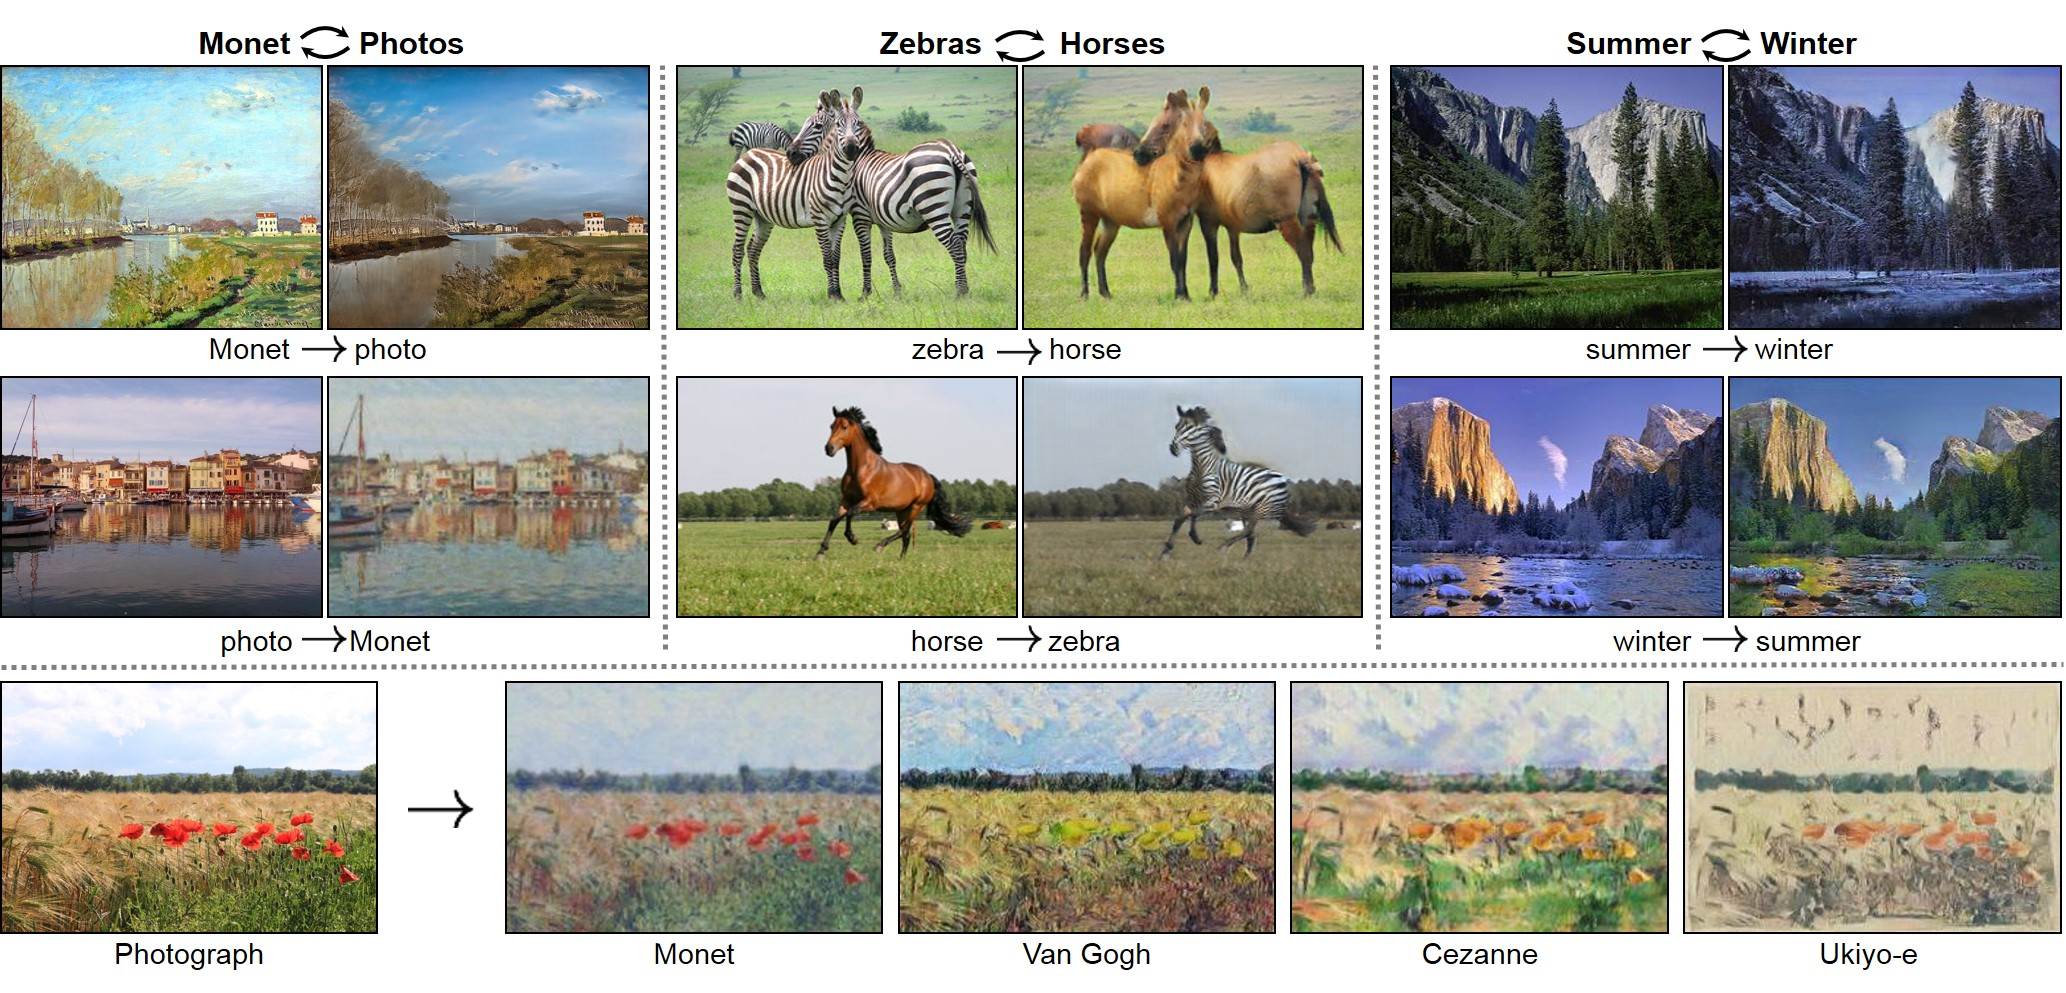
\includegraphics[scale=0.4]{img/gan_img.jpg}
    \end{center}
    \caption{Figure dans le texte~\cite{CycleGAN2017}}
    \label{fig:gan}
\end{figure}
}
\newpage
\appendix

\section{TUTORIEL POUR L'ANNEXE \#1}\label{appendix:consigne}
\begin{enumerate}
    \item Exemples d’informations pouvant figurer dans les annexes : photos, croquis, figures et schémas, tableaux de données, fiche de relevés, etc.
    \item S’il y lieu, les calculs doivent apparaître en annexe (une seule annexe pour tous les calculs du rapport). Il est important de donner clairement les hypothèses de calculs, de citer les références des formules employées et de donner les valeurs des diverses variables et les résultats des calculs.
    \item  S’il y a lieu, inclure des annexes supplémentaires pour consigner les photocopies de catalogues sur des produits particuliers, la correspondance avec les clients ou fournisseurs, les tableaux de résultats, les formulaires divers, les plans de fabrication, résultats de simulation ou autres.
    \item  Il faut désigner les annexes de façon à ce que l’on puisse identifier son contenu (ex. : Annexe B : Spécifications techniques). En pratique, on sépare les annexes par des onglets d’identification. Chaque page d’une annexe est numérotée (ex. : B1, B2, …) et on retrouve au début de chaque annexe une liste du contenu. Attention de ne pas multiplier les annexes à outrance.
\end{enumerate}
Chaque annexe est annoncée deux fois :
\begin{enumerate}
    \item Dans la table des matières;
    \item Dans le corps du rapport, sous la forme d’un renvoi.
\end{enumerate}

Pour citer votre annexe dans le texte, il suffit d'utiliser la commande \ref{appendix:consigne}. De même pour \ref{appendix:fastbook}. La configuration de ce document permet d'inclure directement votre annexe dans la table des matières

\section{TUTORIEL POUR L'ANNEXE \#2}\label{appendix:fastbook}
\begin{center}
    
\includegraphics[scale=1.3]{img/fastbook.png}
\end{center}

\newpage
\bibliographystyle{IEEEtran}
% « La bibliographie est la seule chose que vous pouvez structurer en anglais
% notamment les références IEEE qui ont une rigueur stricte. » (Adjoint à la
% coordination des stages)
\bibliography{references}
\note{
\newpage

MIT License

Copyright (c) 2021 Nathaniel D'Amours et 2023 Département des stages.

Ce document a été initialement réalisé par Nathaniel D'Amours puis modifié par le Département des stages pour y faire figurer les différents annotations, distributions des points et consignes attenantes. Le document est mis à disposition des étudiant(e)s avec l'accord des différentes parties.

Permission is hereby granted, free of charge, to any person obtaining a copy
of this software and associated documentation files (the "Software"), to deal
in the Software without restriction, including without limitation the rights
to use, copy, modify, merge, publish, distribute, sublicense, and/or sell
copies of the Software, and to permit persons to whom the Software is
furnished to do so, subject to the following conditions:

The above copyright notice and this permission notice shall be included in all
copies or substantial portions of the Software.

THE SOFTWARE IS PROVIDED "AS IS", WITHOUT WARRANTY OF ANY KIND, EXPRESS OR
IMPLIED, INCLUDING BUT NOT LIMITED TO THE WARRANTIES OF MERCHANTABILITY,
FITNESS FOR A PARTICULAR PURPOSE AND NONINFRINGEMENT. IN NO EVENT SHALL THE
AUTHORS OR COPYRIGHT HOLDERS BE LIABLE FOR ANY CLAIM, DAMAGES OR OTHER
LIABILITY, WHETHER IN AN ACTION OF CONTRACT, TORT OR OTHERWISE, ARISING FROM,
OUT OF OR IN CONNECTION WITH THE SOFTWARE OR THE USE OR OTHER DEALINGS IN THE
SOFTWARE.
}
\end{document}